\section{Testing algorithms}

Overview of linearisability testing framework. 

Note, assumes deterministic specification object. 

Desirable outcome: no false errors; real errors detected with high probability
(given enough tests).  Distinguish between the real history, in terms of calls
and returns from operations, and the corresponding log, which might contain
delays.  

%%%%%%%%%%%%%%%%%%%%%%%%%%%%%%%%%%%%%%%%%%%%%%%%%%%%%%%

\subsection{Hacking the linearisablity framework}

Can we encode synchronisation linearisability within the linearisability
tester, using the correspondence of the previous section?  Jonathan to think
about this.  Will need to perform two log additions for some concrete
operations.

The idea of linearisability testing is as follows.  We run several threads,
performing operations (typically chosen randomly) upon the concurrent datatype
that we are testing, and logging the calls and returns.  More precisely, a
thread that performs a particular operation~$\sm{op}(x)$: (1) writes
$\call.\sm{op}(x)$ into the log; (2)~performs $\sm{op}(x)$ on the
synchonisation object, obtaining result~$y$, say; (3)~writes $\return.\sm{op}
\:: y$ into the log.  Once all threads have finished, we can use an algorithm
to test whether the history is linearisable.  This can be repeated many times.

Note that there is potentially a delay between writing the $\call$ event into
the log and actually calling the operation; and likewise there is potentially
a delay between the operation returning and writing the $\return$ event into
the log.  However, these delays do not generate false errors: if a history
without such delays is linearisable, then so is a corresponding history with
delays.  Our experience is that the delays do not prevent the detection of
bugs when they exist (although might require performing the test more times). 

It turns out that we cannot use linearisability testing directly with the
specification object~|TwoLinSpec| from Section~\ref{sec:twoStepLinSpec}.  The
obvious way to try to do this would be as follows.  A thread that performs the
concrete operation~$\sm{op}_1(x_1)$: (1)~writes $\call.\sm{op}_1^i(x_1)$ into
the log; (2)~performs $\sm{op}_1(x_1)$ on the synchonisation object, obtaining
result~$y_1$; (3)~writes $\return.\sm{op}_1^i \:: ()$,\,
$\call.\overline{\sm{op}}_1^i()$ and $\return.\overline{\sm{op}}_1^i \:: y_1$
into the log.  A thread that performs operation~|op|\s2 acts as for standard
linearisation testing.  Once all threads have finished, we can use the
existing algorithms for testing whether the history is linearisable with
respect to |TwoStepLinSpec|.

This approach does not work, because it gives false errors.  For example, the
timeline below depicts a log that could be obtained from a correct synchronous
channel using the above approach, where we treat |send| as |op|\s1.
%
\begin{center}
\unScalaMid
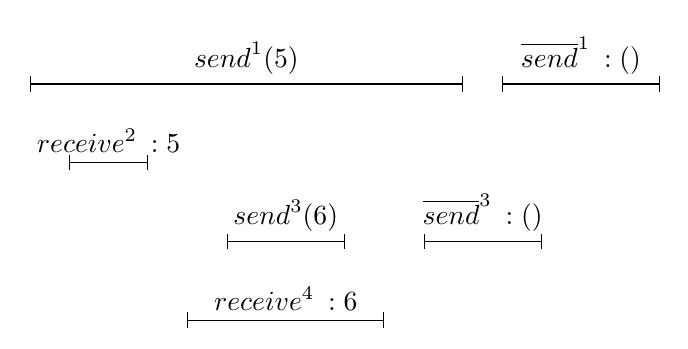
\begin{tikzpicture}
\draw[|-|] (0,0) -- node[above] {  $\sm{send}^1(5)$ } (5.5,0);
\draw[|-|] (6,0) -- node[above] { $\overline{\sm{send}}^1 \:: ()$ } (8,0);
\draw[|-|] (0.5,-1) -- node[above] { $\sm{receive}^2 \:: 5$} (1.5,-1) ;
\draw[|-|] (2.5,-2) -- node[above] {  $\sm{send}^3(6)$ } (4,-2);
\draw[|-|] (5,-2) -- node[above] { $\overline{\sm{send}}^3 \:: ()$ } (6.5,-2);
\draw[|-|] (2.0,-3)  -- node[above] { $\sm{receive}^4 \:: 6$} (4.5,-3);
\end{tikzpicture}
\scalaMid
\end{center}
%
Here, the top two threads synchronise to transmit~5, and then the bottom two
threads synchronise to transmit~6.  However, the top thread is slow to write
its last three events into the log.  The above history is not linearisable
with respect to |TwoStepLinSpec|: this would require $\overline{\sm{send}}^1$
to be linearised before $\sm{send}^3(6)$.  Hence the approach would generate a
false error.

Instead we use a technique that is robust against delays in logging.  We
assume that each thread has an identity in some range $\range 0
{\sm{NumThreads}}$.  We arrange for this identity to be included in the
$\call$ events written to the log for operations~|op|\s1 and
$\overline{\sm{op}}_1$, but otherwise threads act as above.  In particular,
this means that for each thread, calls to~|op|\s1 and $\overline{\sm{op}}_1$
alternate.

We then test whether the history is linearisable with respect to the
specification object below.  It requires that corresponding invocations
of~|op|\s1 and~|op|\s2 are linearised consecutively, but allows the
corresponding $\overline{\sm{op}}_1$ to be linearised later (but before the
next operation invocation by the same thread).  It uses an array |returns|,
indexed by thread identities, to record values that should be returned by a
$\overline{\sm{op}}_1$ operation.
%
\begin{scala}
type ThreadID = Int               // Thread identifiers
val NumThreads: ThreadID = ... // Number of threads
trait State
case class Zero extends State
case class One(t: ThreadID, x£\s1£: A£\s1£) extends State

object TwoStepDelayedLinSpec{
  private var state: State = Zero
  private val returns = new Array[B£\s1£](NumThreads)
  def op£\s1£(t: ThreadID, x£\s1£: A£\s1£): Unit = {
    require(state.isInstanceOf[Zero]); state = One(t, x£\s1£)
  }
  def op£\s2£(x£\s2£: A£\s2£): B£\s2£ = {
    require(state.isInstanceOf[One]); val One(t, x£\s1£) = state
    val (y£\s1£, y£\s2£) = SyncSpec.sync(x£\s1£, x£\s2£); returns(t) = y£\s1£; state = Zero
  }
  def £$\overline{\sm{op}}_1$£(t: ThreadID): B£\s1£ = returns(t) 
}
\end{scala}

In order to argue for correctness, we need to distinguish between:
%
\begin{itemize}
\item the \emph{invocation history}, in terms of actual calls and returns of
  |op|\s1 and |op|\s2; and

\item the corresponding \emph{log history}, which might contain delays.
\end{itemize}
%
Further, the invocation history uses events of the form
$\call.\sm{op}_1^{i_1}(x_1)$,\, $\return.\sm{op}_1^{i_1} \:: y_1$,\,
$\call.\sm{op}_2^{i_2}(x_2)$,\, and $\return.\sm{op}_2^{i_2} \:: y_2$; and the
log history uses events of the form $\call.\sm{op}_1^{i_1}(t,x_1)$ (note the
additional thread identity parameter), $\return.\sm{op}_1^{i_1} \:: ()$ (note
the unit return value), $\call.\overline{\sm{op}}_1^{i_1}(t)$,\,
$\return.\overline{\sm{op}}_1^{i_1} \:: y_1$ (note the transferred return
value), $\call.\sm{op}_2^{i_2}(x_2)$, and $\return.\sm{op}_2^{i_2} \:: y_2$

We can consider the interleaving of the histories, following real-time order.
In the interleaving, for |op|\s1 and |op|\s2,\, $\call$ events from the log
history may be earlier than the corresponding $\call$ events from the
invocation history; and $\return$ events from the log history may be later
than the corresponding $\return$ events from the invocation history.  However,
the two histories agree on the relative order of the |op|\s1 and |op|\s2 events
of each individual thread.

The lemma below shows that this testing method does not generate any false
errors. 
%
\begin{lemma}
Suppose a complete invocation history~$h$ is synchronisation linearisable with
respect to |syncSpec|.  Then each corresponding log history~$h_l$ is
linearisable with respect to |TwoStepDelayedLinSpec|.
\end{lemma}

\begin{proof}
\framebox{**} Non-complete history

Consider the invocation history~$h$ and a corresponding log history~$h_l$; and
consider their real-time interleaving.  By assumption, there is a legal
history~$h_s$ of |SyncSpec| such that $h$ and~$h_s$ are synchronisation
compatible.  Thus $h_s$ may be interleaved with the interleaving of~$h$
and~$h_l$, so that each $\sm{sync}$ event from~$h_s$ is placed between the
corresponding $\call$ and $\return$ events from~$h$, and hence also between
the corresponding $\call$ and $\return$ events from~$h_l$.

We build an interleaving of $h$, $h_l$ and a legal history $h_s'$ of
|Two|\-|Step|\-|Delayed|\-|LinSpec| from the interleaving of~$h$, $h_l$
and~$h_s$, as follows.
%
\begin{enumerate}
\item First, we replace each $\sm{sync}^{i_1,i_2}(x_1,x_2) \:: (y_1,y_2)$ by
  the two (consecutive) events $\sm{op}_1^{i_1}(t,x_1) \:: ()$ and
  $\sm{op}_2^{i_2}(x_2) \:: y_2$, where $t$ is the identity of the thread that
  makes the corresponding call of |op|\s1 in~$h_l$.  
  %% These are between the corresponding $\call$ and $\return$ events
  %% from~$h_l$ for each of $\sm{op}_1^{i_1}$ and $\sm{op}_2^{i_2}$, by
  %% construction.  Further, the relative order of all such events is the same
  %% as the order of the corresponding |sync| events, as required by
  %% |TwoStepDelayedLinSpec|; and the value of each~$y_2$ also agrees with
  %% |TwoStepDelayedLinSpec|.  Finally, the appropriate value~$y_1$ is written
  %% into $\sm{returns}(t)$.

\item Secondly, we insert an event $\overline{\sm{op}}_1^{i_1}(t) \:: y_1$
  between every $\call.\overline{\sm{op}}_1^{i_1}(t)$ and
  $\return.\overline{\sm{op}}_1^{i_1} \:: y_1$ (from~$h_l$), but not between
  any pair of $\sm{op}_1$ and $\sm{op}_2$ events from the previous stage.
  %% Because of the way logging is done, the value of~$y_1$ must match the value
  %% returned by the previous invocation of~|op|\s1 on the synchronisation object
  %% by thread~$t$; and this value much match the last value written into
  %% $\sm{returns}(t)$.  This again agrees with |TwoStepDelayedLinSpec|.
\end{enumerate}
%
Note that each inserted event is between the corresponding $\call$ and
$\return$ events from~$h_l$, by construction.  Let $h_s'$ be these inserted
events; we show that $h_s'$ is a legal history of
|Two|\-|Step|\-|Delayed|\-|LinSpec|.  
\begin{itemize}
\item The events inserted in step~1 alternate between |op|\s1 and~|op|\s2, as
  required by |Two|\-|Step|\-|Delayed|\-|LinSpec|.  Further, they are in the
  same order, and have the same value for~$y_2$, as the corresponding |sync|
  events from~$h_s$.  Hence each inserted |op|\s2 event has the return
  value~$y_2$ as required by |Two|\-|Step|\-|Delayed|\-|LinSpec|.  Finally the
  value $y_1$ written into $\sm{returns}(t)$ (by~|op|\s2 in
  |Two|\-|Step|\-|Delayed|\-|LinSpec|) matches the value returned by the
  corresponding call to~|sync|.

\item For the events from step~2, because of the way logging is done, each
  value of~$y_1$ returned by $\overline{\sm{op}}_1$ must match the value
  returned by the previous invocation of~|op|\s1 on the synchronisation object
  by thread~$t$.  Since~$h$ is synchronisation linearisable, this $y_1$ must
  match the value returned by the corresponding call of~|sync|.  And this
  matches the last value written into $\sm{returns}(t)$ (by the previous
  item), as required by |Two|\-|Step|\-|Delayed|\-|LinSpec|.
\end{itemize}

%
%% Thus the events inserted form a legal history $h_s'$ of
%% |Two|\-|Step|\-|Delayed|\-|Lin|\-|Spec|, with each event between the
%% corresponding $\call$ and $\return$ events from~$h_l$.  
This demonstrates that
$h_l$ is linearisable with respect to |Two|\-|Step|\-|Delayed|\-|LinSpec|.
\end{proof}

%%%%%%%%%%

In theory, the delays in logging may mean that an invocation history that is not
synchronisation linearisable is transformed into a log history that is
linearisable with respect to |Two|\-|Step|\-|Delayed|\-|LinSpec| (although
this seems unlikely).  However, if the delays are sufficiently small, the
log history agrees with the invocation history on the |op|\s1 and~|op|\s2
events.  We show that in this case that log history is not linearisable.
%
\begin{lemma}
Consider an invocation history~$h$ that is not synchronisation linearisable
with respect to $SyncSpec$.  Let $h_l$ be a corresponding log~history that
agrees with~$h$ on |op|\s1 and~|op|\s2 events.  Then $h_l$ is not linearisable
with respect to |Two|\-|Step|\-|Delayed|\-|LinSpec|.
\end{lemma}

%%%%%

\begin{proof}
We prove the contrapositive: we suppose that $h_l$ is linearisable with
respect to |Two|\-|Step|\-|Delayed|\-|LinSpec|, and show that $h$ is
synchronisation linearisable with respect to $SyncSpec$.  

\end{proof}


%%%%%%%%%%%%%%%%%%%%%%%%%%%%%%%%%%%%%%%%%%%%%%%%%%%%%%% 

\subsection{Case with state}

Suppose the specification object has non-trivial state. 

I think it will be more efficient to give a more direct implementation.
Define a configuration to be: (1)~a point in the log reached so far; (2)~the
set of pending operation invocations that have not synchronised; (3)~the set
of pending operation invocations that have synchronised (but not returned);
and (4)~the state of the sequential synchronisation object.  In any
configuration, can: synchronise a pair of pending operations (and update the
synchronisation object); advance in the log if the next event is a return that
is not pending; or advance in the log if the next event is a call.  Then
perform DFS.

Partial order reduction: a synchronisation point must follow either the
call of one of the concurrent operations, or another synchronisation
point.  Any synchronisation history can be transformed into this form, by
moving synchronisation points earlier, but not before any of the corresponding
call events, and preserving the order of synchronisations.  This means that
after advancing past the call of an invocation, we may synchronise that
invocation, and then an arbitrary sequence of other invocations. 

Alternatively, a synchronisation point must precede either the return of one
of the concurrent operations, or another synchronisation point.  This is more
like the JIT technique in the linearisability testing paper.  This means that
before advancing in the log to the return of an invocation that has not
synchronised, we synchronise some invocations, ending with the one in
question.  And we only synchronise in these circumstances. 

My intuition is that the former is more efficient: in the latter, we might
investigate synchronising other invocations even though the returning
operation can't be synchronised with any invocation.  

%%%%%

\subsubsection*{Complexity}

Consider the problem of testing whether a given concurrent history has
synchronisations consistent with a given sequential specification object. 

We make use of a result from~\cite{???} concerning the complexity of the
corresponding problem for linearizability.  Let |Variable| be a
linearizability specification object corresponding to a variable with |get|
and |set| operations.  Then the problem of deciding whether a given concurrent
history is linearisable with respect to |Varaiable| is NP-complete.

Let |ConcVariable| be a concurrent object that represents a variable.  

We consider concurrent synchronisation histories on an object with the
following signature.   
\begin{scala}
object VariableSync{
  def op£\s1£(op: String, x: Int): Int
  def op£\s2£(u: Unit): Unit
} 
\end{scala}
%
The intention is that |op|\s1|("get", x)| acts like |get(x)|, and
|op|\s1|("set", x)| acts like |set(x)| (but returns -1).  The |op|\s2
invocations do nothing except synchronise.  This can be captured formally by
the following synchronisation specification object.

\begin{scala}
object VariableSyncSpec{
  private var state = 0
  def sync((op, x): (String, Int), u: Unit): (Int, Unit) = 
    if(op == "get") (state, ()) else{ state = x; (-1, ()) }
}
\end{scala}


Let |ConcVariable| be a concurrent object that represents a variable.  Given a
concurrent history~$h$ of |ConcVariable|, we build a concurrent history~$h'$
of |VaraibleSync| as follows.  We replace every call or return of |get(x)| by
(respectively) a call or return of |op|\s1|("get", x)|; and we do similarly
with |set|s.  If there are $k$ calls of |get| or |set| in total, we prepend
$k$ calls of |op|\s2, and append $k$ corresponding returns (in any order).
Then it is clear that $h$ is linearisable with respect to |Variable| if and
only if $h'$ is linearisable with respect to |VariableSyncSpec|.

%%%%%%%%%%%%%%%%%%%%%%%%%%%%%%%%%%%%%%%%%%%%%%%%%%%%%%%%%%%%

\subsection{Stateless case}

In the stateless case, a completely different algorithm is possible.  Define
two invocations to be compatible if they could be synchronised, i.e.~they
overlap and the return values agree with those for the specification object.
For $n$ invocations of each operation (so a history of length~$4n$), this can
be calculated in $O(n^2)$.  Then find if there is a total matching in the
corresponding bipartite graph, using the Ford-Fulkerson method, which is
$O(n^2)$.
